\documentclass{cours}
\usepackage{pgfplots}
\usepackage{multicol}
\usepackage{amssymb}
\usepackage{xr}
\usepackage{fontawesome}
\usepackage[inline]{asymptote}
\usetikzlibrary {decorations.text, backgrounds, intersections}
\usepackage{mhchem}

\externaldocument[]{19-premier_principe}
\begin{document}


\setcounter{chapter}{21}
\chapter{Solides cristallins}

Dans ce chapitre, nous allons nous intéresser aux solides cristallins, c'est-à-dire aux solides qui présentent un ordre à grande distance. On commencera par présenter le modèle du cristal parfait puis nous étudierons plus précisément des cristaux métalliques, covalents et ioniques.
    
\section{Modèle du cristal parfait}%
\label{sec:modele_du_cristal_parfait}

\subsection{Définition}%
\label{sub:definition}
\begin{definition}
  Un \textbf{cristal parfait} est un solide de dimension infinie dans lequel les atomes occupent des positions parfaitement périodiques dans l'espace.
\end{definition}

Un cristal parfait est parfaitement défini par un \emph{réseau cristallin} et un \emph{motif}.   

Un réseau cristallin est un ensemble de points répartis périodiquement dans l'espace. Il est défini par 3 vecteurs $\vv{a}$, $\vv{b}$ et $\vv{c}$, et le points du réseau se trouvent aux positions 
\begin{equation}
  R_{ijk}=i \vv{a} + j \vv{b} + k \vv{c} \quad \text{avec} \quad (i, j, k)\in \mathbb{Z}^3\, .
\end{equation}
On passe d'un point à un autre par des translations suivant les vecteurs $\vv{a}$, $\vv{b}$ et $\vv{c}$.  
\begin{center}
  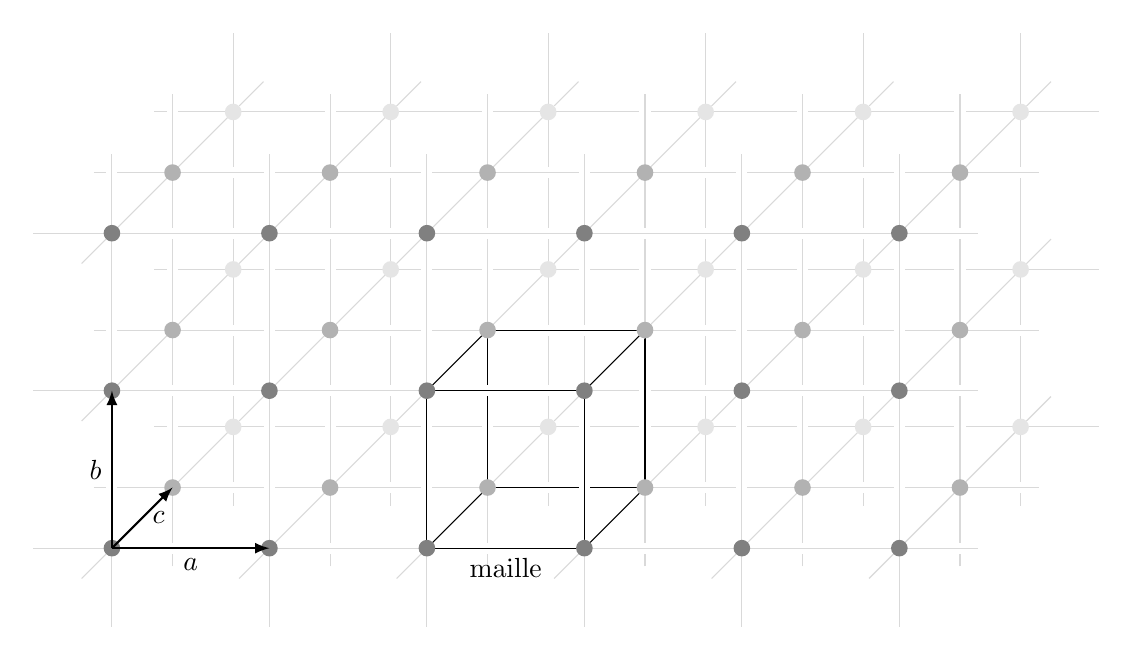
\begin{tikzpicture}
    \tikzset{grille/.style={gray!30, thin, preaction={draw, line width=4pt, white}}}
    \foreach \i in {0,2,...,10}{
      \foreach \j in {0,2,4}{
        \draw[grille] (\i, \j, -1) -- (\i, \j, 5);
      }
    }
    \foreach \k in {0,2,4}{
    \foreach \j in {0,2,4}{
        \draw[grille] (-1, \j, \k) -- (11, \j, \k);
      }
    \foreach \i in {0,2,...,10}{
        \draw[grille] (\i, -1, \k) -- (\i, 5, \k);
        }
    }
    
    \tikzset{maille/.style={preaction={draw, line width=4pt, white}}}
    \draw[maille] (4,0,2) -- (6,0,2) -- (6,2,2) -- (4, 2, 2) -- (4,0,2);
    \draw[maille] (4,0,4) -- (6,0,4) -- (6,2,4) -- (4, 2, 4) -- (4,0,4);
    \draw[maille] (4,0,4) -- (4,0,2)
                  (6,0,4) -- (6,0,2)
                  (4,2,4) -- (4,2,2)
                  (6,2,4) -- (6,2,2);
    \draw (5,0,4) node[below] {maille};
    \foreach \i in {0,2,...,10}{
    \foreach \j in {0,2,4}{
    \foreach \k in {0,2,4}{
    \pgfmathparse{(\k)*20+20}
      \fill[gray!\pgfmathresult] (\i, \j, \k) circle(3pt); 
    }
    }
    }

    \draw[thick, -latex] (0,0, 4) -- node[below]{$\vv{a}$ }++(2,0,0) ;
    \draw[thick, -latex] (0,0, 4) --node[left]{$\vv{b}$ } ++(0,2,0) ;
    \draw[thick, -latex] (0,0, 4) -- node[right]{$\vv{c}$ }++(0,0,-2) ;

  \end{tikzpicture}
  \captionof{figure}{Réseau cristallin pour lequel on a mis en évidence une maille parallélépipédique.}
\end{center}

Pour former le cristal, on place en chaque point du réseau un \textbf{motif} constitué d'un ou plusieurs atomes situés à des positions arbitraires dans la maille. On illustre dans la figure ci-dessous un exemple de réseau et de motif pour un cristal en 2D.  

\begin{center}
  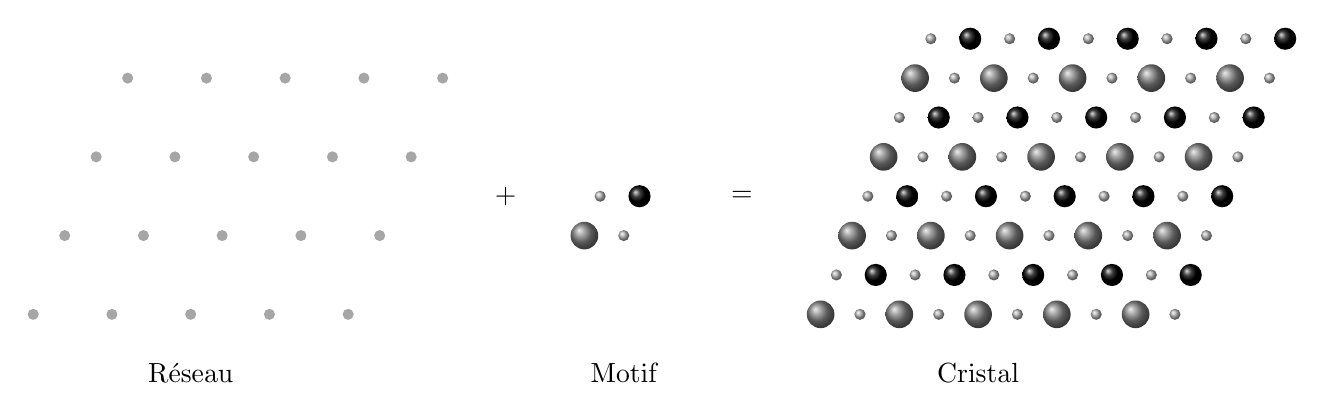
\begin{tikzpicture}
  %tikz%
  % Cristallo, cfc
  %tikz%
    \tikzset{reseau/.style={x=1cm, y={(0.4cm, 1cm)}}}
    
    \foreach \i in {0,1,...,4}{
    \foreach \j in {0,1,...,3}{
      \fill[gray!70, reseau] (\i, \j) circle(2pt); 
    }
    }
    \draw (2,-0.5) node[below] {Réseau};
    \draw (6, 1.5) node{$+$};

    \begin{scope}[xshift=7cm, yshift=1cm] 
      \shade[ball color=gray, reseau] (0, 0) circle (5pt);
      \shade[ball color=black, reseau] (0.5, 0.5) circle (4pt);
      \shade[ball color=gray!60, reseau] (0.5, 0) circle (2pt);
      \shade[ball color=gray!60, reseau] (0, 0.5) circle (2pt);
    \end{scope}
    \draw (7.5,-0.5) node[below] {Motif};
    \draw (9 ,1.5) node{$=$};

    \begin{scope}[xshift=10cm] 
    \foreach \i in {0,1,...,4}{
    \foreach \j in {0,1,...,3}{
      \shade[ball color=gray, reseau] (\i, \j) circle (5pt);
      \shade[ball color=black, reseau] (\i+0.5, \j+0.5) circle (4pt);
      \shade[ball color=gray!60, reseau] (\i+0.5, \j+0) circle (2pt);
      \shade[ball color=gray!60, reseau] (\i+0, \j+0.5) circle (2pt);
    }
    }
    \end{scope}
    \draw (12,-0.5) node[below] {Cristal};


  \end{tikzpicture}
  \captionof{figure}{Construction d'un cristal parfait à partir d'un réseau cristallin et d'un motif.}
\end{center}


\subsection{Caractéristiques d'un cristal parfait}%
\label{sub:caracteristiques_d_un_cristal_parfait}

La \textbf{population} d'une maille d'un cristal parfait est le nombre moyen de chaque type d'atome par maille du cristal. Pour déterminer la population, il faut compter les atomes d'une maille avec un coefficient qui prend en compte le fait que certains atomes sont partagés par plusieurs mailles :
\begin{itemize}
  \item Un atome à l'intérieur de la maille n'appartient qu'à cette maille, il comptera donc pour 1 ;
  \item un atome situé sur une face de la maille est partagé par 2 mailles, il comptera donc pour $\frac{1}{2}$ ;
  \item un atome situé sur une arête de la maille est partagé par 4 mailles, il comptera donc pour $\frac{1}{4}$ ;
  \item un atome situé sur un coin de la maille est partagé par 8 mailles, il comptera donc pour $\frac{1}{8}$.  
\end{itemize}


Par exemple, le rutile est un minéral composé de titane et d'oxygène dont la maille est représentée ci-dessous :
\begin{center}
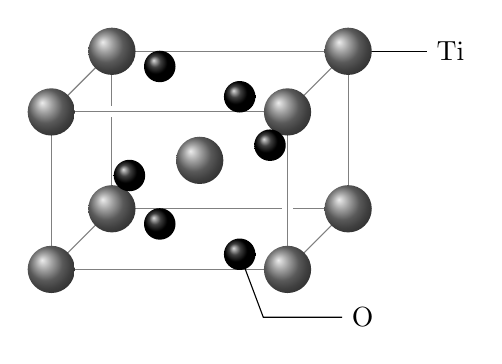
\begin{tikzpicture}
  %tikz  Cristallo, cfc
    \tikzset{maille/.style={preaction={draw, line width=4pt, white}, thin, gray}}
    \draw[maille] (0,0,0) -- (3,0,0) -- (3,2,0) -- (0, 2, 0) -- (0,0,0);
    \draw[maille] (0,0,2) -- (3,0,2) -- (3,2,2) -- (0, 2, 2) -- (0,0,2);
    \draw[maille] (0,0,0) -- (0,0,2)
                  (3,0,0) -- (3,0,2)
                  (3,2,0) -- (3,2,2)
                  (0,2,0) -- (0,2,2);

  \draw (3,2,0) -- ++(1,0) node[right]{$\ce{Ti}$ };
  \draw (2.2,0,1.5) -- ++(0.3,-0.8) --++(1,0) node[right]{$\ce{O}$ };

  \foreach \x in {0,3}{
  \foreach \y in {0,2}{
  \foreach \z in {0,2}{
  \shade[ball color=gray] (\x,\y,\z) circle(0.3cm); 
  }}}
  \shade[ball color=gray] (1.5, 1, 1) circle (0.3cm);

  \foreach \y in {0,2}{
  \shade[ball color=black] (0.8,\y,0.5) circle(0.2cm); 
  \shade[ball color=black] (2.2,\y,1.5) circle(0.2cm); 
  }
  \shade[ball color=black] (2.2,1,0.5) circle(0.2cm); 
  \shade[ball color=black] (0.8,1,1.5) circle(0.2cm); 
\end{tikzpicture}
\captionof{figure}{Structure cristalline du rutile}
\label{fig:rutile}
\end{center}

La population de  cette maille est :
\begin{itemize}
  \item 8 atomes de titane aux coins de la maille, soit $8 \times \frac{1}{8}= 1$ atome de titane ;
  \item 1 atome de titane au centre de la maille, soit $1 \times 1 = 1$ atome de titane ;
  \item 4 atomes d'oxygène sur des faces de la maille, soit $4\times\frac{1}{2}= 2$ atomes d'oxygène ;  
  \item 2 atomes d'oxygène dans la maille, soit $2\times 1 = 2$ atomes d'oxygène.
\end{itemize}
Soit au total 2 atomes de titane et 4 atomes d'oxygène par maille. La formule du rutile est \ce{Ti2O4} que l'on notera \ce{TiO2}. La formule chimique d'un cristal donne les proportions de chaque atome, pas les nombres d'atomes dans le cristal (qui est théoriquement de taille infinie).


La \textbf{coordinence} d'un atome A dans un cristal correspond au nombre d'atomes avec lesquels l'atome A est en contact, ou encore le nombre d'atomes plus proches voisins de l'atome A. Par exemple, dans le rutile dont la structure est présentée sur la figure~\ref{fig:rutile}, chaque atome de titane est entouré de 6 atomes d'oxygène (la coordinence du titane est de 6) et chaque atome d'oxygène est entouré de trois atomes de titane, leur coordinence est donc de 3.

La \textbf{compacité} d'un cristal correspond au rapport du volume occupé par les atomes du cristal sur le volume total du cristal. On peut écrire la compacité $c$ comme
\begin{equation}
  c= \frac{V_\text{atomes}}{V_\text{maille}}
\end{equation}
où $V_\text{atomes}$ est le volume occupé par les atomes d'une maille et $V_\text{maille}$ est le volume d'une maille.

La \textbf{masse volumique} $\rho$ du cristal est le rapport de la masse du cristal sur son volume, on peut aussi l'écrire comme 
\begin{equation}
  \rho = \frac{m_\text{atomes}}{V_\text{maille}}
\end{equation}
où $m_\text{atomes}$ est la masse totale des atomes contenus dans une maille et $V_\text{maille}$ est le volume d'une maille.


\subsection{Limites}%
\label{sub:limites}
Le modèle du cristal parfait n'est, comme son nom l'indique, qu'un modèle, il permet de décrire assez précisément un certain nombre de propriétés des cristaux réels, mais les cristaux réels ne sont \textbf{jamais} des cristaux parfaits. Par exemple :
\begin{itemize}
  \item Les cristaux réels sont toujours finis, ils ont des bords où la structure des atomes ne peu plus être périodique dans l'espace. La structure cristalline de la surface d'un cristal est bien différente de sa structure interne.

  \item Les cristaux réels présentes très souvent des imperfections de périodicité spatiale. Il peut s'agir de \textbf{dislocations}, de la présence d'impuretés ou de lacunes.
\end{itemize}

\begin{center}
  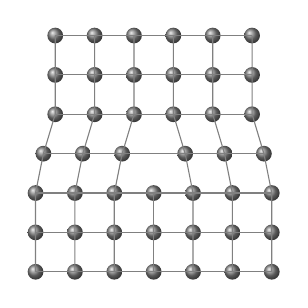
\begin{tikzpicture}[scale=0.5]
  %tikz  Cristallo, cfc
    \foreach \x in {0,1,...,6}{
      \foreach \y in {0,1,...,2}{
        \shade[ball color=gray] (\x,\y) circle(0.2cm);
      }
    }
    \foreach \x in {0,1,...,5}{
      \foreach \y in {0,1,...,2}{
        \shade[ball color=gray] (0.5+\x,4+\y) circle(0.2cm);
      }
    }
    \foreach \x in {0,1,...,2}{
        \shade[ball color=gray] (0.2+\x,3) circle(0.2cm);
        \draw[thin, gray](\x, 0) -- (\x, 2) --(\x+0.2, 3) -- (\x+0.5, 4) -- (\x+0.5, 6);
    }
    \foreach \x in {3,4,...,5}{
        \shade[ball color=gray] (0.8+\x,3) circle(0.2cm);
        \draw[thin, gray](1+\x, 0) -- (1+\x, 2) --(\x+0.8, 3) -- (\x+0.5, 4) -- (\x+0.5, 6);
    }
    \draw[thin, gray] (3,0) -- (3,2);
    \foreach \y in {0,1,2}{
      \draw[thin, gray] (0,\y) -- (6, \y);
    }
    \foreach \y in {4,5,6}{
      \draw[thin, gray] (0.5,\y) -- (5.5, \y);
    }
    \draw[thin, gray] (0.2,3) -- (5.8, 3);
  \end{tikzpicture}
  \captionof{figure}{Exemple de dislocation qui peut apparaître dans un cristal réel.}
\end{center}

\section{Métaux et cristaux métalliques}%
\label{sec:metaux_et_cristaux_metalliques}

\subsection{Liaison métallique et propriétés des métaux}%
\label{sub:liaison_metallique_et_proprietes_des_metaux}


La cohésion des métaux est assurée par la \textbf{liaison métallique}. Cette liaison peut être vue comme une liaison covalente totalement délocalisée, c'est à dire que les électrons de liaison sont délocalisés sur l'ensemble du cristal et libres de s'y déplacer. La liaison métallique est non directionnelle, elle n'a pas de direction privilégiée comme une liaison covalente localisée.

Dans un métal, la présence d'\textbf{électrons libres} est responsable de sa bonne conductivité électrique et thermique, ainsi que de l'aspect réfléchissant du métal.

La non directionnalité de la liaison métallique explique que les métaux soient souvent \textbf{ductiles} (se déforment sans se rompre sous l'effet de la traction) et \textbf{malléables} (se déforment sans se rompre sous l'effet de forces de compression). Elle explique aussi que la plupart des métaux cristallisent dans des structures très compactes, ce qui donne aux métaux une masse volumique élevée.

La liaison métallique est une \textbf{liaison forte}, l'énergie de liaison (entre \num{100} et \SI{800}{\kilo\joule\per\mole}) est cependant un peu plus faible que l'énergie d'une liaison covalente localisée. Cela explique les températures d'ébullition élevées de la plupart des métaux (les liaisons métalliques subsistent à l'état liquide, la température de fusion n'est donc pas un bon indicateur de l'énergie de liaison métallique). 

Dans un métal, on peut modéliser les atomes par des sphères dures qui se touchent, cela permet de définir le \textbf{rayon métallique} des atomes qui composent le métal.

\subsection{Maille cubique faces centrées (CFC)}%
\label{sub:maille_cubique_faces_centrees_cfc}
Nous avons vu que les métaux cristallisent souvent dans des structures compactes, c'est à dire des structures dans lesquelles les atomes sont très proches les uns des autres. Par exemple le cuivre cristallise dans une structure \textbf{cubique faces centrées}, c'est-à-dire que la maille du cristal est cubique et comporte un atome de cuivre à chaque coin ainsi qu'un atome de cuivre au centre de chaque face. 

\begin{center}
  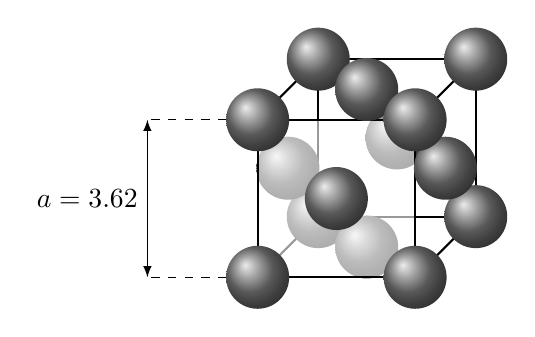
\begin{tikzpicture}[scale=2, baseline={(0,0)}]
  %tikz  Cristallo, cfc
    \def\rr{0.2cm}
    \draw[thick](0,0,0) -- (1,0,0) -- (1, 1, 0) -- (0, 1, 0) --cycle;
    \draw[thick](0,0,0) -- (0, 0, 1);
    \draw[thick](1,0,0) -- (1, 0, 1);
    \draw[thick](0,1,0) -- (0, 1, 1);
    \draw[thick](1,1,0) -- (1, 1, 1);
    \shade[ball color=gray] (0,0,0) circle (\rr);
    \shade[ball color=gray] (1,0,0) circle (\rr);
    \shade[ball color=gray] (1,1,0) circle (\rr);
    \shade[ball color=gray] (0,1,0) circle (\rr);
    \shade[ball color=gray] (0,1/2,1/2) circle (\rr);
    \shade[ball color=gray] (1/2,1/2,0) circle (\rr);
    \shade[ball color=gray] (1/2,0,1/2) circle (\rr);
    \draw[thick, fill=white, fill opacity=0.6](0,0,1) -- (1,0,1) -- (1, 1, 1) -- (0, 1, 1) --cycle;
    \shade[ball color=gray] (1,1/2,1/2) circle (\rr);
    \shade[ball color=gray] (1/2,1/2,1) circle (\rr);
    \shade[ball color=gray] (1/2,1,1/2) circle (\rr);
    \shade[ball color=gray] (0,0,1) circle (\rr);
    \shade[ball color=gray] (1,0,1) circle (\rr);
    \shade[ball color=gray] (1,1,1) circle (\rr);
    \shade[ball color=gray] (0,1,1) circle (\rr);
    \draw[dashed] (-0.2,0,1) -- ++(-0.5,0,0) coordinate (A);
    \draw[dashed] (-0.2,1,1) -- ++(-0.5,0,0) coordinate (B);
    \draw[latex-latex] (A) -- (B) node[midway, left]{$a=\SI{3.62}{\angstrom}$};
  \end{tikzpicture}
  \hspace{4cm}
  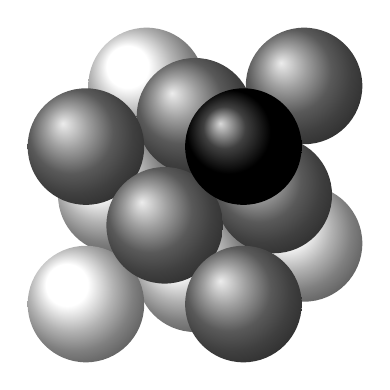
\begin{tikzpicture}[scale=2, baseline={(0,0)}]
  %tikz  Cristallo, cfc
    \def\r{0.37cm}
    \shade[ball color=gray] (0,0,0) circle (\r);
    \shade[ball color=white] (1,0,0) circle (\r);
    \shade[ball color=gray] (1,1,0) circle (\r);
    \shade[ball color=white] (0,1,0) circle (\r);
    \shade[ball color=white] (0,1/2,1/2) circle (\r);
    \shade[ball color=white] (1/2,1/2,0) circle (\r);
    \shade[ball color=white] (1/2,0,1/2) circle (\r);
    \shade[ball color=gray] (1,1/2,1/2) circle (\r);
    \shade[ball color=gray] (1/2,1,1/2) circle (\r);
    \shade[ball color=white] (0,0,1) circle (\r);
    \shade[ball color=gray] (0,1,1) circle (\r);
    \shade[ball color=gray] (1/2,1/2,1) circle (\r);
    \shade[ball color=gray] (1,0,1) circle (\r);
    \shade[ball color=black] (1,1,1) circle (\r);
  \end{tikzpicture}
  \captionof{figure}{Maille cubique faces centrées du cuivre et mise en évidence de l'empilement compact qui la produit (à droite).}
\end{center}
Dans la structure CFC du cuivre, chaque atome de cuivre est en contact avec 12 autres atomes de cuivre. La \textbf{coordinence} du cuivre dans cette structure est donc de 12.

\begin{center}
  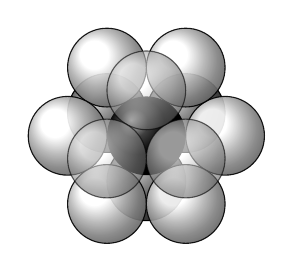
\begin{tikzpicture}
  %tikz  Cristallo, cfc
    \def\rr{0.5}
    \foreach \a in {30, 150, 270}{
      \shade[ball color=gray, opacity=1, draw] (\a:{\rr*2/sqrt(3)}) circle(\rr);
    }
    \shade[ball color=black] (0,0) circle(\rr);
    \foreach \a in {0,60,...,300}{
      \shade[ball color=white, opacity=0.9, draw] (\a:2*\rr) circle(\rr);
      }
    \foreach \a in {-30, 90, 210}{
      \shade[ball color=white, opacity=0.6, draw] (\a:{\rr*2/sqrt(3)}) circle(\rr);
    }
  \end{tikzpicture}
\captionof{figure}{Représentation des 12 plus proches voisins de l'atome noir central dans une structure CFC.}
\end{center}

On peut également déterminer la \textbf{compacité} de cette structure. 
\begin{center}
  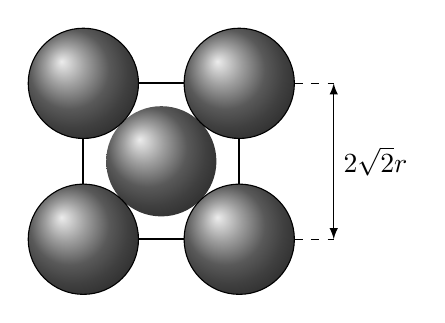
\begin{tikzpicture}
  %tikz  Cristallo, cfc
  \def\rr{0.7}
    \draw[thick] (45:2*\rr) -- (135:2*\rr) -- (225:2*\rr) -- (315:2*\rr) -- cycle;
    \shade[ball color=gray](0,0)  circle (\rr);
    \foreach \a in {45,135,225,315}{
      \shade[ball color=gray, draw] (\a:2*\rr)  circle (\rr);
    }
    \draw[dashed] (45:2*\rr) ++ (\rr, 0) -- ++ (0.5, 0) coordinate (A); 
    \draw[dashed] (315:2*\rr) ++ (\rr, 0) -- ++ (0.5, 0) coordinate (B); 
    \draw[latex-latex] (A) -- (B) node[midway, right]{$2\sqrt{2}r$}; 
  \end{tikzpicture}
  \captionof{figure}{Dimension de la maille cfc en fonction du rayon $r$ d'un atome.}
  \label{fig:dimcfc}
\end{center}
Le volume d'une maille est 
\begin{equation}
  V_\text{maille} = (2\sqrt{2}r)^3 = 16 \sqrt{2}r^3
\end{equation}
Or, une maille comporte 6 atomes sur ses faces et 8 atomes aux coins, ce qui correspond à $n=6\times\frac{1}{2}+8\times\frac{1}{8} = 4$ atomes. Le volume occupé par les atomes est donc 
\begin{equation}
  V_\text{atomes} = 4\times \frac{4}{3}\pi r^3
\end{equation}
et la compacité de la maille est :
\begin{equation}
  c = \frac{V_\text{atomes}}{V_\text{maille}} = \frac{16 \pi r^3}{3 \times 16 \sqrt{2}r^3} = \frac{\pi}{3 \sqrt{2}} \approx \luaexec{SI(math.pi/3/2^0.5, 2, "")}
\end{equation}
C'est la compacité maximale d'un cristal avec un seul type d'atome.

La connaissance du paramètre de maille $a=\SI{3.62}{\angstrom}$ permet aussi de déterminer le \textbf{rayon métallique} de l'atome de cuivre (voir figure~\ref{fig:dimcfc})
\begin{equation}
  r = \frac{a}{2 \sqrt{2}} \approx \luaexec{SI(3.62/2/2^0.5, 2, "\\angstrom")}
\end{equation}

Enfin, connaissant la masse d'un atome de cuivre $m_\text{cuivre}=\luaexec{SIe(63.546*_m_p, 2, "\\kilo\\gram")}$ on détermine la \textbf{masse volumique} $\rho$ du cuivre :
\begin{equation}
  \rho = \frac{m_\text{maille}}{V_\text{maille}} = \frac{4m_\text{cuivre}}{a^3} \approx \luaexec{SIe(4*63.546*_m_p/(3.62e-10)^3, 2, "\\kilo\\gram\\per\\cubic\\meter")}
\end{equation}

\subsection{Sites interstitiels de la maille CFC}%
\label{sub:sites_intersticiels_de_la_maille_cfc}
La compacité de la maille CFC étant inférieure à 1, il reste des espaces vides qui peuvent éventuellement accueillir d'autres atomes, on les appelle des \textbf{sites interstitiels}.

Dans une maille CFC, il existe deux types de sites interstitiels : les \textbf{sites tetraédriques} et les \textbf{sites octaédriques}.

Les \textbf{sites tetraédriques} sont les espaces vides entourés de 4 atomes. Il y en a 8 à l'intérieur de chaque maille, près des coins du cube.

\begin{minipage}{\linewidth}
\begin{center}
  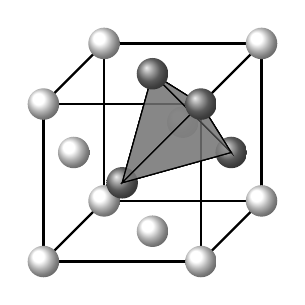
\begin{tikzpicture}[scale=2, baseline={(0,0)}]
  %tikz  Cristallo, cfc
    \def\rr{0.1cm}
    \coordinate(A) at (1,1/2,1/2);
    \coordinate(B) at (1/2,1/2,1);
    \coordinate(C) at (1/2,1,1/2);
    \coordinate(D) at (1,1,1);
    \shade[ball color=white] (1/2,1/2,0) circle (\rr);
    \draw[fill=gray, fill opacity=0.5] (A) -- (B) -- (C) -- cycle;
    \draw[fill=gray, fill opacity=0.5] (D) -- (B) -- (C) -- cycle;
    \draw[fill=gray, fill opacity=0.5] (D) -- (A) -- (C) -- cycle;
    \draw[fill=gray, fill opacity=0.5] (D) -- (A) -- (B) -- cycle;
    \draw[thick](0,0,0) -- (1,0,0) -- (1, 1, 0) -- (0, 1, 0) --cycle;
    \draw[thick](0,0,1) -- (1,0,1) -- (1, 1, 1) -- (0, 1, 1) --cycle;
    \draw[thick](0,0,0) -- (0, 0, 1);
    \draw[thick](1,0,0) -- (1, 0, 1);
    \draw[thick](0,1,0) -- (0, 1, 1);
    \draw[thick](1,1,0) -- (1, 1, 1);
    \shade[ball color=white] (0,0,0) circle (\rr);
    \shade[ball color=white] (1,0,0) circle (\rr);
    \shade[ball color=white] (1,1,0) circle (\rr);
    \shade[ball color=white] (0,1,0) circle (\rr);
    \shade[ball color=white] (0,1/2,1/2) circle (\rr);
    \shade[ball color=white] (1/2,0,1/2) circle (\rr);
    \shade[ball color=gray] (1,1/2,1/2) circle (\rr); %
    \shade[ball color=gray] (1/2,1/2,1) circle (\rr); %
    \draw[fill=gray, fill opacity=0.5] (A) -- (B) -- (C) -- cycle;
    \draw[fill=gray, fill opacity=0.5] (D) -- (B) -- (C) -- cycle;
    \draw[fill=gray, fill opacity=0.5] (D) -- (A) -- (C) -- cycle;
    \draw[fill=gray, fill opacity=0.5] (D) -- (A) -- (B) -- cycle;
    \shade[ball color=gray] (1/2,1,1/2) circle (\rr); %
    \shade[ball color=white] (0,0,1) circle (\rr);
    \shade[ball color=white] (1,0,1) circle (\rr);
    \shade[ball color=gray] (1,1,1) circle (\rr); %
    \shade[ball color=white] (0,1,1) circle (\rr);
  \end{tikzpicture}
  \hspace{4cm}
  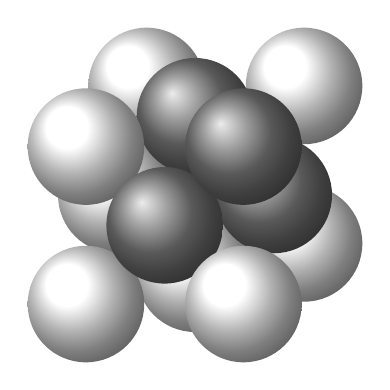
\begin{tikzpicture}[scale=2, baseline={(0,0)}]
  %tikz  Cristallo, cfc
    \def\r{0.37cm}
    \shade[ball color=white] (0,0,0) circle (\r);
    \shade[ball color=white] (1,0,0) circle (\r);
    \shade[ball color=white] (1,1,0) circle (\r);
    \shade[ball color=white] (0,1,0) circle (\r);
    \shade[ball color=white] (0,1/2,1/2) circle (\r);
    \shade[ball color=white] (1/2,1/2,0) circle (\r);
    \shade[ball color=white] (1/2,0,1/2) circle (\r);
    \shade[ball color=gray] (1,1/2,1/2) circle (\r);
    \shade[ball color=gray] (1/2,1,1/2) circle (\r);
    \shade[ball color=white] (0,0,1) circle (\r);
    \shade[ball color=white] (0,1,1) circle (\r);
    \shade[ball color=gray] (1/2,1/2,1) circle (\r);
    \shade[ball color=white] (1,0,1) circle (\r);
    \shade[ball color=gray] (1,1,1) circle (\r);
  \end{tikzpicture}
  \captionof{figure}{Position d'un site tetraédrique (en gris) de la structure CFC.}
\end{center}
\end{minipage}

L'\textbf{habitabilité} d'un site interstitiel correspond au rayon maximal d'un atome qui peut s'y introduire sans le déformer. Nous allons déterminer l'habitabilité d'un site tétraédrique.

On commence par remarquer que les quatre sommets d'un site tétraédrique se trouve aux coins d'un cube de côté $\frac{a}{2}$, où $a$ est le paramètre de la maille.

\begin{center}
  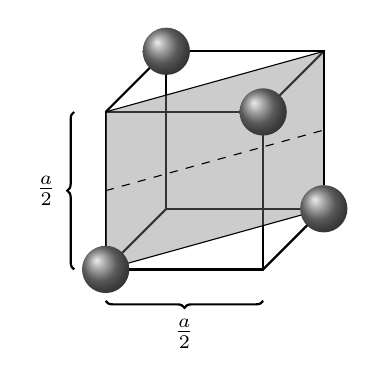
\begin{tikzpicture}
  %tikz  Cristallo, cfc
    \pgfmathsetmacro{\r}{2/sqrt(2)};
    \draw[thick] (0,0,0) -- (2, 0, 0) -- (2, 2, 0) -- (0,2, 0) --cycle; 
    \draw[thick] (0,0,2) -- (2, 0, 2)  -- (2, 2, 2) -- (0,2, 2) --cycle; 
    \draw[thick](0,0,0) -- (0, 0, 2);
    \draw[thick](2,0,0) -- (2, 0, 2);
    \draw[thick](0,2,0) -- (0, 2, 2);
    \draw[thick](2,2,0) -- (2, 2, 2);
    \def\dd{0.0}
    \def\aa{2}
    \draw[fill=gray, fill opacity=0.4](0,\aa, \aa) -- ++ (\aa+\dd, 0, -\aa-\dd) -- ++(0, -\aa, 0) -- ++(-\aa-\dd, 0, +\aa+\dd) --cycle;
    \draw[dashed] (0,1,2) -- (2, 1,0 );
    \shade[ball color=gray] (0,0,2) circle (0.3);
    \shade[ball color=gray] (2,0,0) circle (0.3);
    \shade[ball color=gray] (2,2,2) circle (0.3);
    \shade[ball color=gray] (0,2,0) circle (0.3);
    \draw[thick,decorate, decoration={brace}](-0.4, 0, 2) -- (-0.4, 2, 2) node[left, xshift=-3, midway]{$\frac{a}{2}$ };
    \draw[thick,decorate, decoration={brace, mirror}](0, -0.4, 2) -- (2, -0.4, 2) node[below, yshift=-3, midway]{$\frac{a}{2}$ };
  \end{tikzpicture}
  \hspace{3cm}
  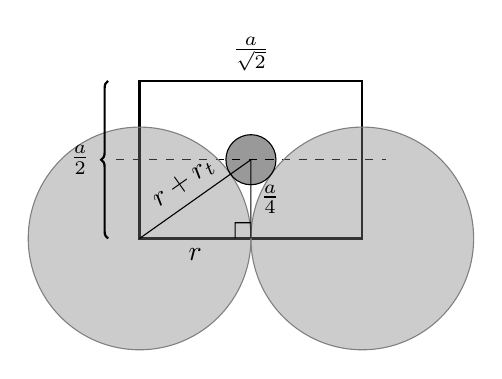
\begin{tikzpicture}
  %tikz  Cristallo, cfc
    \pgfmathsetmacro{\r}{2/sqrt(2)};
    \pgfmathsetmacro{\rt}{(sqrt(3)-sqrt(2))};
    \draw[thick] (0,0) rectangle (2*\r, 2);
    \draw[dashed] (-0.3, 1) -- (2*\r+0.3, 1);
    \draw[gray, fill, fill opacity=0.4] (0,0) circle(\r);
    \draw[gray, fill, fill opacity=0.4] (2*\r,0) circle(\r);
    \draw[black, fill, fill opacity=0.4] (\r,1) circle(\rt);
    \draw (\r, 2) node[above]{$\frac{a}{\sqrt{2}}$};  
    \draw[thick,decorate, decoration={brace}](-0.4, 0) -- (-0.4, 2) node[left, xshift=-3, midway]{$\frac{a}{2}$ };
    \draw (0,0) --  node[sloped, above]{$r+r_t$} (\r, 1) -- node[right]{$\frac{a}{4}$}(\r, 0) ++ (-0.2, 0) --++(0, 0.2) --++(0.2, 0);
    \draw (\r/2, 0) node[below]{$r$}; 
  \end{tikzpicture}
  \captionof{figure}{Éléments de calcul de l'habitabilité d'un site tétraédrique. Pour des raisons de symétrie, l'atome inséré, de rayon maximum $r_t$  dans le site tétraédrique se trouve forcément au milieu du site.}
  \label{fig:calcultetra}
\end{center}

Sur la figure~\ref{fig:calcultetra}, on peut déterminer le rayon maximum de l'atome inséré dans le site tétraédrique par :
\begin{equation}
  (r+r_t)^2 = \left( \frac{a}{4} \right) ^2 + r^2 \quad \text{soit} \quad r_t = \sqrt{\frac{a^2}{16}+ r^2}-r
\end{equation}

En utilisant $r=\frac{a}{2 \sqrt{2}}$, on trouve l'habitabilité du site tétraédrique :
\begin{equation}
  r_t = a \left( \sqrt{\frac{1}{16}+\frac{1}{8}} - \frac{1}{2 \sqrt{2}} \right)  = a \frac{\sqrt{3}-\sqrt{2}}{4} \approx \luaexec{SI(362*(3^0.5-2^0.5)/4,1, "\\pico\\meter")} 
\end{equation}

Les sites octaédriques sont des espaces vides entourés de 6 atomes. Dans une maille cubique faces centrées, il y a un site octaédrique au centre de la maille, et un quart de site tetraédrique sur chaque arête (voir figure~\ref{fig:site_octa}).
\begin{center}
  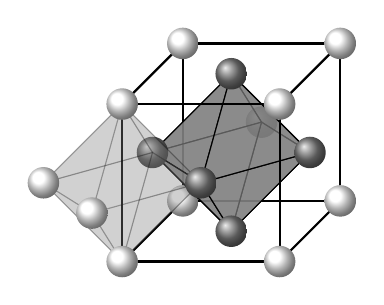
\begin{tikzpicture}[scale=2, baseline={(0,0)}]
  %tikz  Cristallo, cfc
    \def\rr{0.1cm}
    \coordinate(A) at (1/2,1/2,1);
    \coordinate(B) at (1,1/2,1/2);
    \coordinate(C) at (1/2,1/2,0);
    \coordinate(D) at (0,1/2,1/2);
    \coordinate(E) at (1/2,1,1/2);
    \coordinate(F) at (1/2,0,1/2);

    \draw[thick](0,0,0) -- (1,0,0) -- (1, 1, 0) -- (0, 1, 0) --cycle;
    \draw[thick](0,0,0) -- (0, 0, 1);
    \draw[thick](1,0,0) -- (1, 0, 1);
    \draw[thick](0,1,0) -- (0, 1, 1);
    \draw[thick](1,1,0) -- (1, 1, 1);

    \shade[ball color=gray] (1/2,1/2,0) circle (\rr);
    \shade[ball color=white] (0,0,0) circle (\rr);
    \draw[fill=gray, fill opacity=0.7] (B) -- (C) -- (E) -- cycle;
    \draw[fill=gray, fill opacity=0.7] (C) -- (D) -- (E) -- cycle;
    \draw[fill=gray, fill opacity=0.7] (B) -- (C) -- (F) -- cycle;
    \draw[fill=gray, fill opacity=0.7] (C) -- (D) -- (F) -- cycle;
    \draw[fill=gray, fill opacity=0.7] (D) -- (A) -- (E) -- cycle;
    \draw[fill=gray, fill opacity=0.7] (D) -- (A) -- (F) -- cycle;
    \draw[fill=gray, fill opacity=0.7] (B) -- (A) -- (F) -- cycle;
    \draw[fill=gray, fill opacity=0.7] (B) -- (A) -- (E) -- cycle;

    \draw[thick](0,0,1) -- (1,0,1) -- (1, 1, 1) -- (0, 1, 1) --cycle;

    \shade[ball color=gray] (0,1/2,1/2) circle (\rr);
    \draw[fill=gray, opacity=0.2] (D) -- (A) -- (0,1,1) -- cycle;
    \draw[fill=gray, opacity=0.2] (D) -- (A) -- (0,0,1) -- cycle;
    \draw[fill=gray, opacity=0.2] (A) -- (0,0,1) -- (0, 1/2, 1.5) -- cycle;
    \draw[fill=gray, opacity=0.2] (A) -- (0,1,1) -- (0, 1/2, 1.5) -- cycle;
    \draw[fill=gray, opacity=0.2] (-0.5, 0.5, 1) -- (0,1,1) -- (0, 1/2, 1.5) -- cycle;
    \draw[fill=gray, opacity=0.2] (-0.5, 0.5, 1) -- (0,0,1) -- (0, 1/2, 1.5) -- cycle;
    \draw[fill=gray, opacity=0.2] (-0.5, 0.5, 1) -- (0,0,1) -- (D) -- cycle;
    \draw[fill=gray, opacity=0.2] (-0.5, 0.5, 1) -- (0,1,1) -- (D) -- cycle;
    \shade[ball color=white, opacity=1] (-0.5,0.5,1) circle (\rr);
    \shade[ball color=white, opacity=1] (0,0.5,1.5) circle (\rr);


    \shade[ball color=white] (1,0,0) circle (\rr);
    \shade[ball color=white] (1,1,0) circle (\rr);
    \shade[ball color=white] (0,1,0) circle (\rr);
    \shade[ball color=gray] (1/2,0,1/2) circle (\rr);
    \shade[ball color=gray] (1,1/2,1/2) circle (\rr); 
    \shade[ball color=gray] (1/2,1/2,1) circle (\rr); 
    \shade[ball color=gray] (1/2,1,1/2) circle (\rr); 
    \shade[ball color=white] (0,0,1) circle (\rr);
    \shade[ball color=white] (1,0,1) circle (\rr);
    \shade[ball color=white] (1,1,1) circle (\rr); 
    \shade[ball color=white] (0,1,1) circle (\rr); 

  \end{tikzpicture}
  \hspace{4cm}
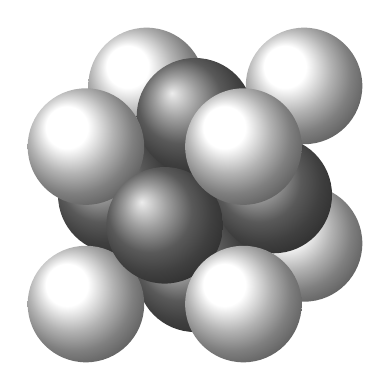
\begin{tikzpicture}[scale=2, baseline={(0,0)}]
  %tikz  Cristallo, cfc
    \def\r{0.37cm}
    \shade[ball color=white] (0,0,0) circle (\r);
    \shade[ball color=white] (1,0,0) circle (\r);
    \shade[ball color=white] (1,1,0) circle (\r);
    \shade[ball color=white] (0,1,0) circle (\r);
    \shade[ball color=gray] (0,1/2,1/2) circle (\r);
    \shade[ball color=gray] (1/2,1/2,0) circle (\r);
    \shade[ball color=gray] (1/2,0,1/2) circle (\r);
    \shade[ball color=gray] (1,1/2,1/2) circle (\r);
    \shade[ball color=gray] (1/2,1,1/2) circle (\r);
    \shade[ball color=white] (0,0,1) circle (\r);
    \shade[ball color=white] (0,1,1) circle (\r);
    \shade[ball color=gray] (1/2,1/2,1) circle (\r);
    \shade[ball color=white] (1,0,1) circle (\r);
    \shade[ball color=white] (1,1,1) circle (\r);
  \end{tikzpicture}
  \captionof{figure}{Position d'un site octaédrique (en gris) de la structure CFC.}\label{fig:site_octa}
\end{center}

Pour des raisons de symétrie, l'atome le plus gros que l'on puisse placer sur un site octaédrique doit se situer au centre d'une arête. Nous allons déterminer son rayon maximum $r_o$. 

\begin{center}
  
  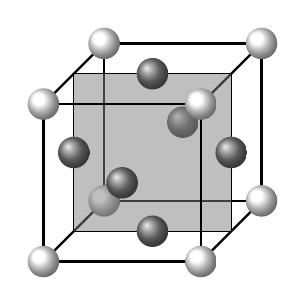
\begin{tikzpicture}[scale=2, baseline={(0,0, 1)}]
  %tikz  Cristallo, cfc
    \def\rr{0.1cm}
    \coordinate(A) at (1/2,1/2,1);
    \coordinate(B) at (1,1/2,1/2);
    \coordinate(C) at (1/2,1/2,0);
    \coordinate(D) at (0,1/2,1/2);
    \coordinate(E) at (1/2,1,1/2);
    \coordinate(F) at (1/2,0,1/2);

    \draw[thick](0,0,0) -- (1,0,0) -- (1, 1, 0) -- (0, 1, 0) --cycle;
    \draw[thick](0,0,0) -- (0, 0, 1);
    \draw[thick](1,0,0) -- (1, 0, 1);
    \draw[thick](0,1,0) -- (0, 1, 1);
    \draw[thick](1,1,0) -- (1, 1, 1);

    \shade[ball color=gray] (1/2,1/2,0) circle (\rr);
    \shade[ball color=white] (0,0,0) circle (\rr);

    \draw[fill=gray, draw,fill opacity=0.5] (0, 0, 0.5) rectangle (1, 1, 0.5);

    \draw[thick](0,0,1) -- (1,0,1) -- (1, 1, 1) -- (0, 1, 1) --cycle;

    \shade[ball color=gray] (0,1/2,1/2) circle (\rr);
    \shade[ball color=white] (1,0,0) circle (\rr);
    \shade[ball color=white] (1,1,0) circle (\rr);
    \shade[ball color=white] (0,1,0) circle (\rr);
    \shade[ball color=gray] (1/2,0,1/2) circle (\rr);
    \shade[ball color=gray] (1,1/2,1/2) circle (\rr); 
    \shade[ball color=gray] (1/2,1/2,1) circle (\rr); 
    \shade[ball color=gray] (1/2,1,1/2) circle (\rr); 
    \shade[ball color=white] (0,0,1) circle (\rr);
    \shade[ball color=white] (1,0,1) circle (\rr);
    \shade[ball color=white] (1,1,1) circle (\rr); 
    \shade[ball color=white] (0,1,1) circle (\rr); 
  \end{tikzpicture}
  \hspace{3cm}
  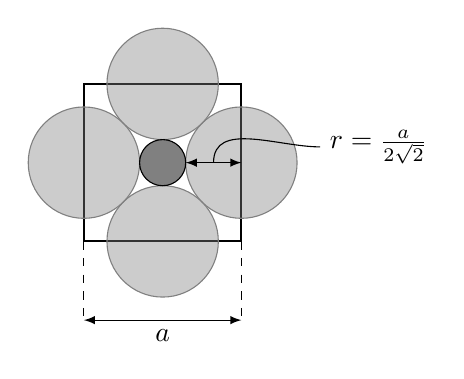
\begin{tikzpicture}[baseline={(0,0)}]
  %tikz  Cristallo, cfc
    \draw[thick] (0,0) rectangle (2,2);
    \draw[gray, fill, fill opacity=0.4] (0,1) circle({1/sqrt(2)}); 
    \draw[gray, fill, fill opacity=0.4] (2,1) circle({1/sqrt(2)}); 
    \draw[gray, fill, fill opacity=0.4] (1,0) circle({1/sqrt(2)}); 
    \draw[gray, fill, fill opacity=0.4] (1,2) circle({1/sqrt(2)}); 

    \draw[dashed] (0,0) -- ++(0, -1) coordinate (A);
    \draw[dashed] (2,0) -- ++(0, -1) coordinate (B);
    \draw[latex-latex] (A) -- node[below]{$a$}(B);
    \draw[latex-latex] ({2-1/sqrt(2)}, 1) -- coordinate (A) (2, 1);
    \draw (A) to[out=90, in=180] (3, 1.2) node[right]{$r=\frac{a}{2 \sqrt{2}}$}; 
    \draw[fill=gray] (1,1) circle({1-1/sqrt(2)});
  \end{tikzpicture}
  \captionof{figure}{Éléments de calcul de l'habitabilité d'un site octaédrique.}
\end{center}
On trouve alors que l'habitabilité d'un site octaédrique est 
\begin{equation}
  r_o = \frac{a}{2}-r = \frac{a}{2} - \frac{a}{2 \sqrt{2}} = \frac{a}{2} \left( 1 - \frac{1}{\sqrt{2}} \right) \approx \luaexec{SI(362/2*(1-1/2^0.5), 1, "\\pico\\meter")}
\end{equation}

\section{Cristaux covalents}%
\label{sec:solides_covalents}
Les cristaux covalents sont des cristaux dont la cohésion est assurée par des liaisons covalentes entre les atomes qui les composent. La liaison covalente est \textbf{forte} et très \textbf{directionnelle}, l'énergie d'une liaison covalente est de l'ordre de 200 à \SI{800}{\kilo\joule\per\mole}. Par exemple, le diamant est un cristal covalent d'atomes de carbone.

La force de la liaison covalente explique la température de fusion élevée (\sim \SI{1000}{\kelvin}) de la plupart des cristaux covalents ainsi que leur dureté. La directionnalité de la liaison covalente explique la faible malléabilité et la faible ductilité des cristaux covalents. 

Dans un modèle de sphères dures, deux atomes $A_1$ et $A_2$   d'un cristal covalent plus proches voisins sont séparés par une distance $d_{12}=r_1+r_2$, où $r_1$ et $r_2$ sont les \textbf{rayons covalents} des deux atomes.

Le diamant est un exemple classique de cristal covalent, il est constitués d'atomes de carbones ayant une structure cubique faces centrées, avec en plus des atomes de carbone qui occupent un site tétraédrique sur deux (voir figure~\ref{fig:diamant})

\begin{center}
    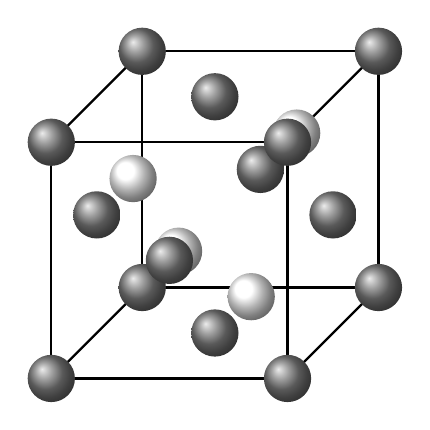
\begin{tikzpicture}[scale=3, baseline={(0,0, 1)}]
  %tikz  Cristallo, cfc
    \def\rr{0.1cm}
    \coordinate(A) at (1/2,1/2,1);
    \coordinate(B) at (1,1/2,1/2);
    \coordinate(C) at (1/2,1/2,0);
    \coordinate(D) at (0,1/2,1/2);
    \coordinate(E) at (1/2,1,1/2);
    \coordinate(F) at (1/2,0,1/2);

    \draw[thick](0,0,0) -- (1,0,0) -- (1, 1, 0) -- (0, 1, 0) --cycle;
    \draw[thick](0,0,0) -- (0, 0, 1);
    \draw[thick](1,0,0) -- (1, 0, 1);
    \draw[thick](0,1,0) -- (0, 1, 1);
    \draw[thick](1,1,0) -- (1, 1, 1);

    \shade[ball color=gray] (1/2,1/2,0) circle (\rr);
    \shade[ball color=gray] (0,0,0) circle (\rr);


    \draw[thick](0,0,1) -- (1,0,1) -- (1, 1, 1) -- (0, 1, 1) --cycle;

    \shade[ball color=gray] (0,1/2,1/2) circle (\rr);
    \shade[ball color=gray] (1,0,0) circle (\rr);
    \shade[ball color=gray] (1,1,0) circle (\rr);
    \shade[ball color=gray] (0,1,0) circle (\rr);
    \shade[ball color=gray] (1/2,0,1/2) circle (\rr);
    \shade[ball color=gray] (1,1/2,1/2) circle (\rr); 
    \shade[ball color=gray] (1/2,1,1/2) circle (\rr); 
    \shade[ball color=white] (0.25,0.75,0.75) circle (\rr); 
    \shade[ball color=white] (0.75,0.75,0.25) circle (\rr); 
    \shade[ball color=white] (0.75,0.25,0.75) circle (\rr); 
    \shade[ball color=white] (0.25,0.25,0.25) circle (\rr); 
    \shade[ball color=gray] (1/2,1/2,1) circle (\rr); 
    \shade[ball color=gray] (0,0,1) circle (\rr);
    \shade[ball color=gray] (1,0,1) circle (\rr);
    \shade[ball color=gray] (1,1,1) circle (\rr); 
    \shade[ball color=gray] (0,1,1) circle (\rr); 
  \end{tikzpicture}
  \captionof{figure}{Structure du diamant, tous les atomes sont des atomes de carbone, on a représenté en blanc les atomes qui occupent les sites tétraédriques de la structure CFC.} 
  \label{fig:diamant}
\end{center}

\section{Cristaux ioniques}%
\label{sec:solides_ioniques}
La cohésion des cristaux ioniques est assurée par l'interaction électrostatique attractive entre les cations et les anions qui composent le cristal.

La liaison ionique est une liaison \textbf{forte} et \textbf{non directionnelle}. L'énergie de liaison ionique est de l'ordre de 100 à \SI{600}{\kilo\joule\per\mole}.

l'intensité de la liaison ionique explique la haute température de fusion et la dureté des cristaux ioniques. La nature ionique de la liaison rend les cristaux ioniques facilement solubles dans les solvants polaires (par exemple dans l'eau).


Un cristal ionique est électriquement neutre. Une maille du cristal doit donc contenir autant de cations que d'anions.

Dans un modèle de sphères dures, les ions d'un cristal ionique plus proches voisins sont séparés par une distance $d=r_+ + r_-$, où $r_+$ et $r_-$ sont les \textbf{rayons ioniques} respectifs du cation et de l'anion.

Le chlorure de sodium est un exemple de cristal ionique. Il a une structure CFC avec les ions chlorures aux n\oe{}uds et les ions sodium sur les sites octaédriques (au centre des arêtes).

\begin{center}
    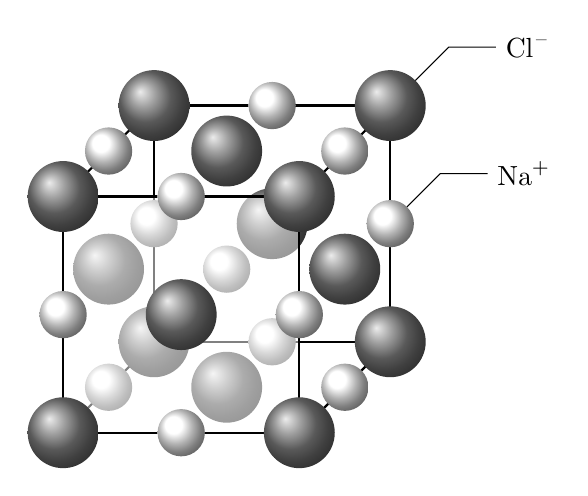
\begin{tikzpicture}[scale=3, baseline={(0,0, 1)}]
  %tikz  Cristallo, cfc
    \def\rr{0.1cm}
    \def\rrCl{0.15cm}
    \coordinate(A) at (1/2,1/2,1);
    \coordinate(B) at (1,1/2,1/2);
    \coordinate(C) at (1/2,1/2,0);
    \coordinate(D) at (0,1/2,1/2);
    \coordinate(E) at (1/2,1,1/2);
    \coordinate(F) at (1/2,0,1/2);

    \draw[thick](0,0,0) -- (1,0,0) -- (1, 1, 0) -- (0, 1, 0) --cycle;
    \draw[thick](0,0,0) -- (0, 0, 1);
    \draw[thick](1,0,0) -- (1, 0, 1);
    \draw[thick](0,1,0) -- (0, 1, 1);
    \draw[thick](1,1,0) -- (1, 1, 1);

    \shade[ball color=gray] (1/2,1/2,0) circle (\rrCl);
    \shade[ball color=gray] (0,0,0) circle (\rrCl);
    \shade[ball color=white] (0.5,1,0) circle (\rr); 
    \shade[ball color=white] (0,0.5,0) circle (\rr); 
    \shade[ball color=white] (1,0.5,0) circle (\rr); 
    \shade[ball color=white] (0.5,0,0) circle (\rr); 

    \shade[ball color=white] (0,1,0.5) circle (\rr); 
    \shade[ball color=white] (0,0,0.5) circle (\rr); 
    \shade[ball color=white] (1,1,0.5) circle (\rr); 
    \shade[ball color=white] (1,0,0.5) circle (\rr); 

    \shade[ball color=white] (0.5,0.5,0.5) circle (\rr); 

    \shade[ball color=gray] (0,1/2,1/2) circle (\rrCl);
    \shade[ball color=gray] (1/2,0,1/2) circle (\rrCl);
    \draw[thick, fill=white, fill opacity=0.5](0,0,1) -- (1,0,1) -- (1, 1, 1) -- (0, 1, 1) --cycle;

    \shade[ball color=gray] (1,0,0) circle (\rrCl);
    \shade[ball color=gray] (1,1,0) circle (\rrCl);
    \shade[ball color=gray] (0,1,0) circle (\rrCl);
    \shade[ball color=gray] (1,1/2,1/2) circle (\rrCl); 
    \shade[ball color=gray] (1/2,1,1/2) circle (\rrCl); 
    \shade[ball color=gray] (1/2,1/2,1) circle (\rrCl); 
    \shade[ball color=gray] (0,0,1) circle (\rrCl);
    \shade[ball color=gray] (1,0,1) circle (\rrCl);
    \shade[ball color=gray] (1,1,1) circle (\rrCl); 
    \shade[ball color=gray] (0,1,1) circle (\rrCl); 
    \shade[ball color=white] (0.5,1, 1) circle (\rr); 
    \shade[ball color=white] (0,0.5,1) circle (\rr); 
    \shade[ball color=white] (1,0.5,1) circle (\rr); 
    \shade[ball color=white] (0.5,0,1) circle (\rr); 

    \draw (1,1,0) ++ (45:\rrCl) -- ++(45:0.2) -- ++(0.2, 0) node[right]{\ce{Cl-}};
    \draw (1,0.5,0) ++ (45:\rr) -- ++(45:0.2) -- ++(0.2, 0) node[right]{\ce{Na+}};
  \end{tikzpicture}
  \captionof{figure}{Structure du chlorure de sodium (\ce{NaCl}).} 
  \label{fig:diamant}
\end{center}
\section{Cristaux moléculaires}%
\label{sec:cristaux_moleculaires}
Dans les cristaux moléculaires, la cohésion est assurée par des liaisons faibles (liaisons hydrogène ou liaisons de Van Der Waals). L'énergie de liaison est de l'ordre de 1 à \SI{10}{\kilo\joule\per\mole} pour les liaisons de Van Der Waals et de 10 à \SI{50}{\kilo\joule\per\mole} pour les liaisons hydrogène. 

La faiblesse des liaisons explique la faible température de fusion des cristaux moléculaires et leur faible dureté. 
Les liaisons hydrogène étant très directionnelles, les cristaux moléculaires qui possèdent ce type de liaisons sont peu maléables et peu ductiles.

Un exemple classique de cristal moléculaire est la glace (eau solide). Les liaisons entre les molécules d'eau sont des liaisons hydrogène. 

\end{document}
